La biogéographie est l'étude de la répartition géographiques des
espèces. Aujourd'hui, ce terme est souvent remplacé par celui de
macroécologie. Outre la distinction historique, ce mot met en avant
l'importance du rapport des espèces à leur environnement (biotique ou
abiotique) plutôt que la dimension évolutive pourtant tout aussi
importante. C'est pour garder à l'esprit la richesse des facteurs qui
dessinent les aires de répartition que je garde le terme de
biogéographie, discipline dont je dresse un portrait dans la présente
introduction. J'y aborde aussi bien la complexité de la compréhension de
la distribution spatiale des espèces que les cadres théoriques associés.
Chemin faisant, je discute de l'importance du lien qu'il existe entre
les interactions écologiques et la répartition des espèces ; cette
réflexion est l'essence même de ma thèse.

\section*{Des îles et des espèces}\label{des-uxeeles-et-des-espuxe8ces}
\addcontentsline{toc}{section}{Des îles et des espèces}

\subsection*{En suivant Wallace}\label{en-suivant-wallace}
\addcontentsline{toc}{subsection}{En suivant Wallace}

Dans l'introduction de son livre \emph{Island Life} paru en 1881, le
célèbre naturaliste Alfred Russel Wallace nous rapporte deux faits
étonnants qui justifient pleinement l'examen attentif de la répartition
géographique des espèces \citep{wallace1881island}. Premièrement, le
biogéographe démontre, à l'aide de nombreux exemples, que l'éloignement
entre deux régions du monde n'est pas suffisant pour conclure quand à
l'éloignement de leur composition faunistique et floristique. Ainsi, la
comparaison des avifaunes du l'île japonaise d'Hokkaido et de
l'Angleterre, séparées par des milliers de kilomètres, révèle une
proximité des paysages ornithologiques très supérieure à celle constatée
dans l'analyse comparée des oiseaux des îles indonésiennes de Bali et de
Lombok pourtant distantes de quelques kilomètres seulement.
Deuxièmement, en s'appuyant sur les différences des faunes brésiliennes
et africaines, Wallace souligne la faiblesse du pouvoir prédictif des
variables climatiques pour décrire les compositions faunistiques
présentes sous des latitudes similaires. Ces constatations soulignent
l'utilité de croiser les informations des distributions à la lumière
d'une analyse taxonomique pour y apporter du sens. Dans le cadre de la
théorie de l'évolution\footnote{Wallace a publié en 1858 un article
  \emph{On the Tendency of Varieties to Depart Indefinitely From the
  Original Type} qui témoigne très clairement que ses idées sur les
  varitions temporelles des espèces étaient très proches de celles de
  Charles Darwin a qui il avait d'ailleurs envoyé son manuscrit
  \citep{Wallace1858}.}, encore toute jeune en 1881, cette analyse
taxonomique est une analyse historique : Wallace montre que la
compréhension d'un problème spatial, celui des aires de répartition de
groupes d'espèces, n'est possible que par une compréhension temporelle,
celle de l'histoire des espèces. Cette idée est clairement énoncée dans
la suite de son introduction :
%
\begin{quote}
« Many years study of this class of subjects has convinced me that there
is no short abd easy method of dealing with them; because they are, in
their very nature, the visible outcome and residual product of the whole
past history of the earth. »
\end{quote}
%
Tout au long de son livre, Wallace démontre que la connaissance à
l'échelle mondiale de la distribution des êtres vivants permet
d'associer les différentes îles aux grands ensembles régionaux
biologiques (que nous appelons aujourd'hui écozones) sur la base des
ressemblances biologiques des espèces qui témoignent du lien temporel
unissant les différentes zones géographiques de la Terre. Ce travail de
caractérisation d'ensemble géographiques conduit notamment Wallace, dans
un article de 1860 \citep{Wallace1860}, à tracer la ligne éponyme
séparant l'écozone indomalaise de l'écozone australienne (séparant les
îles de Bali et Lomonk mentionnée au paragraphe précédent). La
connaissance apportée à la géographie par l'histoire est saisissante et
les exemples de Wallace deviennent autant d'arguments en faveur de la
théorie de l'évolution. Le discours de Wallace porte sur des processus à
des échelles spatiales et temporelles très grandes\footnote{L'âge de la
  terre est très débattu à l'époque. Bien que l'ensemble des savants
  s'accordent pour aller bien au-delà des 6000 ans bibliques, il n'y a
  alors pas de consensus. Wallace affirme à la page 212 du chapitre 10
  de \emph{Island Life} que la vie se développait il y a au moins 500
  millions d'années \citep{wallace1881island}, ce qui est audacieux pour
  l'époque mais bien en-dessous de l'âge des plus anciens fossiles
  découverts à ce jour qui est estimé à 3.4 milliards d'années
  \citep{Wacey2011}.}, ce qui apporte certes un éclairage substantiel
qui se double cependant d'un obstacle épistémologique majeur : si
l'explication ultime de la présence d'une espèce en un point donné est
le produit d'une série de contingences historiques, quelles peuvent être
les fondations d'une théorie de la biogéographie? Ce n'est qu'au
XX\textsuperscript{ème} siècle que des réponses convaincantes
émergeront.
%
\subsection*{En suivant MacArthur et
Wilson}\label{en-suivant-macarthur-et-wilson}
\addcontentsline{toc}{subsection}{En suivant MacArthur et Wilson}

Parmi les visions les plus importantes de la biogéographie ce trouve
celle contenue dans le livre publié en 1967 \emph{The Theory of Island
Biogeography}, produit de la fructueuse rencontre du mathématicien et
biologiste Robert MacArthur et du myrmécologue Edward Wilson\footnote{Cet
  actuel professeur émérite à l'université d'Harvard est reconnu pour
  ses apports en biologie et en sociologue, il est notamment l'auteur de
  32 livres. C'est pour son immense connaissance des fourmis que j'ai
  choisi l'adjectif de myrmécologue.}. A partir d'un grand nombre de
données sur les faunes insulaires de diverses régions du monde, ces
auteurs ont construit un cadre théorique puissant pour expliquer les
variations du nombre d'espèce trouvé sur ces îles \citep{MacArthur1967}.
Leur démarche théorique permet de lier des observations a un modèle
mathématique donnant une explication simple et convaincante des
variations étudiées. Ils font ainsi basculer la discipline dans une ère
nouvelle, ce dont les auteurs étaient conscients, en atteste le premier
paragraphe du dernier chapitre de leur livre :

\begin{quote}
« Biogeography has long remained in a natural history phase,
accumulating information about the distribution of species and higher
taxa and the taxonomic composition of biotas. Interpretative reasoning
has been largely directed to the solution of special problems connected
with the histories of individuals taxa and biotas. Without doubt this
descriptive activity will continue to be of fundamental importance to
the science, one of the most physically adventurous of all scientific
entreprises and, in the richness of the detail it unfolds, esthetically
pleasing. But biogeography is also in a position to enter an equally
interesting experimental and thereotical phase. »
\end{quote}

Dans cet extrait, MacArthur et Wilson affirment que l'étude de la
distribution des espèces doit sortir du royaumes des contingences
historiques pour devenir un objet de science au sens d'être manipulé
aussi bien expérimentalement que par l'abstraction mathématique. La
validation expérimentale de la théorie a d'ailleurs été menée par Wilson
et son étudiant au doctorat de l'époque Daniel Simberloff devenu depuis
un célèbre écologue \citep{Simberloff1969}. Le travail d'abstraction
mathématique a été conduit par MacArthur dans le livre de 1967 et
prolongé dans les annexes de son livre de 1972
\citep{macarthur1972geographical}. Ces auteurs proposent une explication
de la variation spécifique des îles fondée sur deux processus opposés :
la colonisation d'espèce depuis le continent qui augmente le nombre
d'espèce sur l'île et un processus d'extinction locale qui diminue ce
nombre. C'est en reliant ces processus aux propriétés physiques de l'île
(aire et isolation) et en interprétant la richesse spécifique des îles
en terme d'équilibre entre ces deux processus que les auteurs
parviennent à expliquer de manière convaincante les relations observées
entre richesse spécifique, taille de l'île et isolement. Dans le
troisième temps de cette introduction, je reviens amplement sur cette
théorie nommée théorie de la biogéographie des îles que je noterai TIB
dans la suite.

Le paradigme de la TIB est un lègue qui a eu un impact considérable sur
les développements théoriques en écologie \citep{Warren2015}. Au centre
du projet de la TIB se loge la volonté de mettre l'espèce au coeur de la
biogéographie afin de permettre à la discipline de s'enrichir des
mécanismes biologiques qui sont un moteur essentiel de la variation dans
la distribution des espèces. L'intérêt de leur \emph{biogéographie de
l'espèce} (terme donné à l'avant-dernière phrase de leur livre) est dans
l'affirmation qu'il faut regarder les contraintes conjointes de
l'évolution (qui met un certains nombre d'espèces avec des
caractéristiques propres en présence) et du contexte écologique qui
détermine les conditions d'extinction. Cette intrication de l'écologie
et de l'évolution est bien inscrite dans la pensée de MacArthur et
Wilson même si la puissance de leur vision réside dans le fait de les
occulter en partie.

Près de 50 ans après la parution de leur livre, une des clef en biologie
semble être la compréhension des rétroactions qu'il existe entre
écologie et évolution dans les variations spatiales et temporelles de la
biodiversité. Je reprend ci-dessous trois aphorismes cités par
\citet{Schoener2011a} concernant les liens entre biologie, écologie et
évolution :

\begin{quote}
« Nothing in biology makes sense except in the light of evolution. »
\citep{Dobzhansky1973}
\end{quote}

\begin{quote}
« Nothing in evolutionary biology makes sense except in the light of
ecology. » \citep{grant2008}
\end{quote}
%
\begin{quote}
« Nothing in evolution or ecology makes sense except in the light of the
other. » \citep{Pelletier2009a}
\end{quote}

La chronologie de ces citations est un indice de la reconnaissance
actuel du besoin (de la nécessité?) de croiser écologie et évolution. Un
parallèle avec les sciences humaines me semble possible dans lequel
l'écologie serait à la biologie ce que la géographie est aux sciences
humaines et l'évolution serait à la biologie ce que l'histoire est aux
sciences humaines. Nous pouvons certes étudier l'une sans l'autre, mais
le dialogue entre les deux disciplines est indispensable. En son
absence, les disciplines avancent en trainant avec elles des hypothèses
fortes sur l'autre qui finiront éventuellement par nuire à une
compréhension plus profonde de la biologie. Par exemple, supposer que
les variations démographiques ont des origines purement écologiques
devient problématique si les variations génétiques sont suffisantes pour
expliquer qu'une partie importante de cette variation comme cela l'a été
montré sur une population de mutons de Soay \citep{Pelletier2007}. Je ne
cherche pas à nier l'utilité des savoirs acquis de manière autonome par
un champ disciplinaire, j'insiste simplement sur l'importance de mettre
ces connaissances en commun dans une synthèse indispensable pour
décrypter l'information contenue dans les distributions d'espèce.
%
\subsection*{Quelles informations renferment les distributions
d'espèces?}
\addcontentsline{toc}{subsection}{Quelles informations renferment les
distributions d'espèces?}

Cette question est non seulement une invitation à découvrir les raisons
de la présence de tel ou tel organisme en un lieu donné du globe, mais
elle suggère aussi que certaines informations ne peuvent pas être
obtenues par l'analyse de la répartition géographique des espèces. Les
auteurs mentionnés dans les paragraphes précédents y ont apporté des
éléments de réponse cruciaux : Wallace a montré que les distributions
géographiques reflétaient en partie les liens de parenté entre les
espèces, quant à MacArthur et Wilson, ils ont suggérés que ces
distributions étaient le résultat de processus écologiques dynamiques.
Examiner les aires de répartition, en détailler la géométrie exacte et
les variations spatio-temporelle, faire des recoupements entre les
répartitions géographiques de différentes espèces ou encore avec la
distribution de variables abiotiques sont des démarches fondamentales
pour en apprécier les mécanismes sous-jacents.

Dans son ouvrage de 1972, MacArthur discute de l'ensemble de ces
mécanismes, il considère aussi bien le rôle que peuvent jouer les
variables climatiques que celui des interactions écologiques. En plus
des exemples concrets amenés pour illustrer ses propos, MacArthur
développe des modèles mathématiques pour prolonger la discussion. Au
chapitre 2, il formalise l'impact de la compétition sur la coexistence
des espèces aboutissant ainsi sur un principe de ségrégation spatiale
des espèces liées par ce type de relation : deux compétiteurs ne peuvent
pas co-occurrer (résider durablement au même endroit) sauf
éventuellement sur zone très restreinte de leur distribution
\citep{macarthur1972geographical}. Toujours dans cet ouvrage, MacArthur
évoque la distribution en damier (\emph{checkerboard}) que peuvent
générer des espèces en compétition. La discussion sur ce type de
distribution sera approfondie par Jared Diamond \citep{Diamond1975} dont
les travaux déclencheront un débat important sur la determination de
modèle nul de co-occurrence \citep{Connor1979} et sur laquelle ma thèse
apporte quelques éléments nouveaux.

L'étude sur un grand nombre d'espèce de leurs limites spatiales permet
d'y déceler des généralités quant aux mécanismes qui les déterminent
\citep{macarthur1972geographical}. L'examen des variations
spatio-temporelles apporte une information très utile sur l'importance
relative des divers mécanismes. Le contexte des changements climatiques
est une bonne illustration de ce principe car les bouleversements
actuels des répartitions géographiques permettent en effet de pointer le
rôle majeur de certains mécanismes évolutifs auparavant sous-estimés
\citep{Lavergne2010}. Enfin, l'examen des distributions doit aussi être
un examen des co-distributions, il faut s'intéresser à l'information de
sous ensembles d'espèces et notamment les espèces en interaction afin de
tester si la biologie laisse des empreintes dans la géométrie des aires
de répartition. Par exemple, dans ma thèse je propose de regarder
l'intersection des l'aire associée à un ensemble de proies pour savoir
ce qu'elle nous apprend sur la distribution de leur prédateur.

\subsection*{Enjeux de la connaissance de la répartition géographique
des
espèces}\label{enjeux-de-la-connaissance-de-la-ruxe9partition-guxe9ographique-des-espuxe8ces}
\addcontentsline{toc}{subsection}{Enjeux de la connaissance de la
répartition géographique des espèces}

Les observations et la compréhension des causes profondes de la
géométrie et la dynamique des aires de répartitions des espèces ont déjà
amené à des découvertes majeures en écologie et en évolution. La phase
d'expérimentation et de théorisation de la biogéographie décrite par
MacArthur et Wilson se poursuit et se tourne vers un objectif très
ambitieux : faire de la biogéographie une discipline prédictive,
pourvoyeuse de prédictions fiables sur les aires de répartitions futures
de n'importe quelle espèce. Ce problème est d'autant plus présent dans
la littérature récente que nous sommes dans un contexte où ces aires
sont profondément bouleversées. En biogéographie, les changements
climatiques ont en effet canalisés l'attention des chercheurs qui
constatent avec stupeur l'ampleur à laquelle la biodiversité mondiale
est affectée \citep{Koh2004, Bellard2012}. La volonté d'anticiper la
localisation future des espèces a également engendré des efforts
conséquents pour développer des outils statistiques essentiellement
centrés sur la corrélation entre les variables abiotiques et les données
de présence (d'occurrence) des espèces \citep{Elith2006}.
%
En ciblant l'étude de la distribution de certaines espèces, la
biogéographie rencontrent des enjeux socio-économiques majeurs. Ainsi,
pour un pays comme la France, la restriction des zones favorables à la
croissance de la vigne envisagée è l'aide des scénarios de changements
climatique \citep{Hannah2013} pourrait conduire à des pertes économiques
importantes et un bouleversement identitaire des grandes régions
viticoles. De plus, détecter aujourd'hui un potentiel viticole futur
dans des régions où cette production n'existe pas peut conduire à des
augmentations drastiques du prix des terres agricoles. En guise de
second exemple, je pose la question suivant : où seront les érablières
de demain? La réponse est donnée par la détermination de la répartition
future des aires favorables à la croissance de l'érable à sucre
(\emph{Acer saccharum}) et de sa capacité à les atteindre afin de s'y
établir. Je termine avec un troisième exemple : la perte des
pollinisateurs et notamment des abeilles. Pas moins de quatre grandes
classes de facteurs d'origine anthropique les mettent en danger : les
changements climatiques, le changement dans l'utilisation des
terres\footnote{Les changements dans l'utilisations des terres sont
  accompagnés, entre autres, de l'utilisation parfois massive de
  pesticides de la famille des néonicotinoïdes affaiblissant les
  colonies.}, l'apparition de nouveaux pathogènes (dont l'acarien
parasite \emph{Varroa destructoa} vecteur de nombreux virus) et
l'arrivée d'espèces invasives (comme le frelon asiatique)
\citep{Vanbergen2013}. Le défi actuel est de prédire la distribution
future des pollinisateurs en intégrant ces multiples aspects et leurs
interactions. De plus, dans le cas des espèces invasives, il faut
comprendre comment une espèce peut sortir de son aire de répartition
naturelle et en établir une nouvelle.

Actuellement, les outils de prédictions des aires de répartition future
reposent essentiellement sur les scénarios de changements climatiques.
La démarche est cohérente : la connaissance basée sur les corrélations
de variables climatiques permet d'établir une relation climat-présence.
En utilisant les résultats des climatologues qui dérivent les variations
climatiques associées à des scénarios d'émission de gaz a effet de serre
par les activités humaine, les biogéographes établissent les
probabilités de présence des espèces dans les conditions climatiques
futures. Cependant, la relation climat-présence n'est qu'une facette du
lien qui unissent les espèces à l'espace et chaque nouvelle invasion
nous montre à quel point il est difficile de prédire les aires de
répartitions. Ces problèmes de qualité de prédictions sont le reflet de
lacunes théoriques qui amènent plusieurs chercheurs à se positionner en
faveur d'un renouvellement des fondations théoriques pour édifier une
biogéographie plus intégrative
\citep{Lomolino2000, Beck2012, Thuiller2013}. Bien sur, ces appels
soulèvent des défis importants dont on ne peut qu'espérer qu'ils soient
relevés au plus vite pour faire face à l'urgence.

\subsection*{Travail théorique et
modélisation}\label{travail-thuxe9orique-et-moduxe9lisation}
\addcontentsline{toc}{subsection}{Travail théorique et modélisation}

Avant d'énumérer, avec des exemples concrets, l'ensemble des forces qui
régissent la répartition géographique d'une espèce, je souligne dans
cette partie l'importance du travail de théorie et de modélisation qui
joue un rôle prépondérant dans ma thèse.

\subsubsection*{Rassembler et intégrer des
faits}\label{rassembler-et-intuxe9grer-des-faits}
\addcontentsline{toc}{subsubsection}{Rassembler et intégrer des faits}

Le travail de théorie est avant tout la mise en cohésion d'un certain
nombre de faits, d'observations. Dans la TIB, par exemple, MacArthur et
Wilson proposent une explication cohérente de l'augmentation de la
richesse spécifique dans les îles de plus grande taille. Trois principes
encadrent la construction d'une théorie scientifique :

\begin{enumerate}
\def\labelenumi{\arabic{enumi}.}
\item
  la théorie doit pouvoir être testées (par une expérience ou par la
  récolte de données),\\
\item
  la théorie doit être falsifiable : la théorie demeure valide tant
  qu'elle n'est pas prouvée fausse, tant qu'une théorie alternative ne
  la supplante pas,\\
\item
  la théorie doit être parcimonieuse, ne pas invoquer de multiples
  processus sans raison (c'est-à-dire sans une augmentation du nombre de
  faits expliqués), c'est un principe qui est aussi connu sous le nom de
  Rasoir d'Ockham.
\end{enumerate}
%
Une boutade, dont je ne suis pas capable de me souvenir son auteur,
énonce que les physiciens expliquent 95\% de l'univers avec 5 règles
alors que les économistes expliquent 5\% des phénomènes qu'ils étudient
avec 95 règles\footnote{Une variante indique que les économistes ont
  prédit 12 des trois dernières crises économiques. Je pense que pour ce
  qui est de nos capacités de prédictions, la biogéographie est plus
  proche de l'économie que la de la physique..}. Le problème n'est pas
tant de dénigrer une discipline mais de constater d'un côté la puissance
prédictive d'une théorie mature et de l'autre, les problèmes posés par
une théorie lacunaire. En biogéographie, j'ai le sentiment que les
théories manquent de maturité, la TIB donne certes une vision cohérente
de la richesse spécifique insulaire mais c'est une théorie peu précise :
prédire un nombre d'espèce n'aide que partiellement à comprendre le
monde qui nous entoure. Pour faire un peu de prospective, une théorie
qui donnerait des prédictions sur la topologie des réseaux et la
composition en masse des espèces présentes supplanterait la TIB car elle
expliquerait davantage de faits au prix probable d'une complexité
supérieure.

\subsubsection*{Des modèles pour explorer et tester la
théorie}\label{des-moduxe8les-pour-explorer-et-tester-la-thuxe9orie}
\addcontentsline{toc}{subsubsection}{Des modèles pour explorer et tester
la théorie}

Le terme de modèle signifie simplement que l'objet en question à des
propriétés bien connues. Un organisme modèle, par exemple, est un
organisme souvent facile à élever et manipuler pour lequel beaucoup de
connaissances ont été acquises, iL sert souvent d'unité empirique pour
un ou plusieurs groupes de recherche. Les modèles statistiques sont des
outils pour tester des relations basées sur des hypothèses issues de
théories. De même, pour un travail de modélisation mathématique, la
description du modèle est contenu dans une série d'équations dérivée
d'une théorie. A travers les modèles, quelle qu'en soit leur nature on
explore et on teste une théorie que l'on a éventuellement participé à
établir.

Les modèles sont souvent décrits comme une simplification de la réalité
: comment, en effet, prétendre que les mécanismes biologiques décelés
chez \emph{Arabidopsis Thaliana}\footnote{Il s'agit de la plante modèle
  par excellence dont le génome fut le premier à être séquencé chez les
  plantes \citep{TheArabidopsisGenomeInitiative2000}.} sont les mêmes à
l'oeuvre pour l'ensemble des plantes à fleurs? pour combien de systèmes
proie-prédateur le modèle de Lotka-Volterra est-il pertinent? Les
limites des modèles doivent être reconnues mais il ne faut pas nier
l'apport de ces derniers. Les modèles sont autant de chance pour
explorer une ou plusieurs prédiction d'une théorie. Le choix du modèle
employé est lié à l'histoire du chercheur qui l'utilise, à ses
propensions mentales à utiliser avec succès telle ou telle démarche
scientifique, c'est ce que rappelle Kevin McCann dans la préface de son
livre \emph{Food Webs} \citep{mccann2011food}:

\begin{quote}
« It just so happens that some people find it easier to think about
things in terms of x's and y's, and other in terms rabbits of and lynx.
»
\end{quote}

En d'autres termes, certaines personnes ont plus de facilités pour
penser en termes d'abstraction mathématique alors que d'autres font
meilleur usage de manipulations plus concrètes. Je suis plutôt dans la
première catégorie de personne, je pense que les mathématiques sont un
cadre de penser très puissant comme l'indique le grand écologue Robert
May \citep{May2004}:

\begin{quote}
« The virtue of mathematics in such a contexte is that it forces clarity
and precision upon the conjecture, thus enabling meaningful comparison
between the consequences of basics assumptions and the empirical facts.
Here mathematics is seen in its quintesence : no more, but no less, than
a way to think clealy. »
\end{quote}

Dans ma thèse, j'ai essayé d'utiliser les mathématiques pour développer
des modèles dont le point de départ a été une réflexion collective
autour du rôle que pouvaient jouer les interactions dans la répartition
géographique des espèces. J'ai alors établi un cadre théorique avec
lequel j'ai dérivé des prédictions dont certaines semblent être
vérifiées dans les données empiriques.

\subsubsection*{Nouvelles prédictions}\label{nouvelles-pruxe9dictions}
\addcontentsline{toc}{subsubsection}{Nouvelles prédictions}

Après l'établissement d'une théorie expliquant un certain nombre de
faits et pour laquelle un certain nombre de tests ont été réalisés, le
raisonnement fondé sur celle-ci peut conduire à la production de
nouvelles prédictions dont la vérification la renforceront. En revanche,
l'apparition des faits expérimentaux en désaccord avec cette théorie
demanderont des réponses qui se traduiront soit par une meilleur
compréhension de la limite d'application de la théorie soit par
l'émergence d'une théorie nouvelle qui expliquera ces faits nouveaux
tout en couvrant le rayon de compréhension de la théorie précédente. Ces
dernières années, la physique nous a donné deux exemples très probants
du pouvoir de l'imagination avec la vérification expérimentale de
théories énoncées bien avant que les outils permettant de la vérifier
existent. En 2012, c'est la détection du Boson de Higgs dont l'existence
fut prédite en 1964\footnote{Pour plus de détail, je réfère le lecteur
  au bulletin du CERN disponible en ligne
  \url{http://cds.cern.ch/journal/CERNBulletin/2012/28/News\%20Articles/1459456?ln=fr}}.
Cette année, c'est la détection des ondes gravitationnelles soit 100 ans
après qu'Einstein en ait prédit l'existence \citep{Waldrop2016}. En
biogéographie, une théorie devrait être capable, par exemple, de dresser
des cartes d'invasibilité à l'échelle mondiale pour l'ensemble des
espèces. Je pense que nous en sommes encore loin, néanmoins, le chemin
pour y parvenir passe par une connaissance approfondie de l'ensemble des
mécanismes qui interviennent dans le tracé des aires de répartition,
c'est-à-dire connaître leur nature, la portée de leur action mais aussi
leurs interactions et leurs importances relatives.

\section*{Les processus qui façonnenet les aires de
répartition}\label{les-processus-qui-fauxe7onnenet-les-aires-de-ruxe9partition}
\addcontentsline{toc}{section}{Les processus qui façonnenet les aires de
répartition}

\subsection*{Biogéographie
historique}\label{bioguxe9ographie-historique}
\addcontentsline{toc}{subsection}{Biogéographie historique}

Il s'agit de la compréhension des impacts sur les êtres vivants des
évènements de grande amplitude temporelle (allant de quelques milliers
d'années à plusieurs millions d'années). C'est dans l'étude de la
proximité des taxons mais aussi des fossiles éventuels que l'on peut
déchiffrer les mouvements de colonisation des différentes branches de
l'arbre du vivant. Pour prendre un exemple de phénomène de très grande
amplitude, on peut faire appel à la théorie de la dérive des continents
établie par Alfred Lothar Wegener\footnote{La similarité des fossiles
  trouvés sur des continents très éloignés a été un des arguments en
  faveur de cette théorie.} qui implique que des groupes éventuellement
proches il y a des millions d'années ont été séparés et ont donné
naissance à des lignées différentes. Aujourd'hui, nous sommes capables
de retracer ces liens de parenté à l'aide de phylogénies moléculaires
qui sont des outils très efficaces pour estimer le temps que sépare
différents. Ainsi, par la comparaison des génomes mitochondriaux, il a
été montré récemment que les lémuriens (primates malgaches) ont été
séparées de toute autre lignée de primates il y a 60 millions d'année
environs \citep{Finstermeier2013}. Cette séparation questionne bien sur
sur la série d'évènements qui ont conduit à l'isolation de ce groupe de
singes à Madagascar et à la construction des communautés que nous y
observons actuellement \citep{Razafindratsima2013}.

Les processus de grandes amplitudes temporelles sont cependant dominés
par leur composante historique (et donc non reproductible) et prédire
des phénomènes tel que l'extinction des dinosaures est, dans le meilleur
des cas, très compliqué. Néanmoins, dans les mouvements de grandes
amplitudes se manifestent des processus qui sont en permanence à
l'oeuvre. Ainsi, l'étude de la diversification des bousiers entreprise
par Joachim Hortal et collègues \citep{Hortal2011} montre que la
dernière glaciation a laissé des empreintes encore visibles dans la
carte de répartition de la diversité de ce groupe : la limite de la
thermocline 0°C durant le dernier maximum glacier (il y a 21000 ans
environs) sépare les zones de fortes diversifiées en bousier des autres.
De plus, ils montrent que la diversité phylogénique des espèces
nordiques, c'est-à-dire plus tolérantes au froid, est un sous-ensemble
phylogénétique bien identifié, par conséquent peu de branches des
bousiers sont à l'origine des colonisations nordiques. Ainsi, après une
contraction de la zone favorable au développement des bousiers, les
mouvements de colonisation ont marqué à la fois la carte de répartition
de la richesse spécifique de ce groupe mais aussi la carte de la
répartition des différentes branches de l'arbre phylogénétique des
bousiers européens \citep{Hortal2011}.

\subsection*{Capactés de dispersion}\label{capactuxe9s-de-dispersion}
\addcontentsline{toc}{subsection}{Capactés de dispersion}

La remonté nordique des bousiers depuis le dernier maximum glacier est
le résultat d'événements de dispersion individuel. Au cours de leur vie,
les bousiers parcourent de grandes distances à la recherche de
nourriture, on peut imaginer qu'au fil des génération, si les conditions
environnementales le permettent, certains individus établissent des
populations de plus en plus nordiques. Ce qui est vrai pour ce groupe
d'espèce mobile l'est aussi pour des espèces sessiles comme les plantes
qui possèdent également des capacités de dispersion du fait de la
dissémination de leurs semences par des mécanismes très diversifiés. Ce
rapport à l'espace des différents organismes est une forme de diffusion
: des mouvements stochastiques conduisent à une augmentation de la
répartition (c'est une question de probabilité), mais cette diffusion
n'est pas totalement libre.

Plusieurs types de contrainte limitent l'élargissement de l'aire de
répartition d'une espèce. Pour les espèces terrestres, les mers et les
océans sont des obstacles majeurs à la colonisation de nouveaux
territoires. A l'échelle régionale, les rivières, les hauts reliefs
peuvent fortement limiter la dispersion d'une espèce. De même, pour les
plantes dont la stratégie de dissémination est l'anémochorie, la vitesse
et la direction des vents sont des facteurs primordiaux pour comprendre
la propagation de l'espèces. Enfin, à l'échelle du paysage, il existe
très souvent une mosaïque d'habitats plus ou moins favorables à la
dispersion d'une espèce. Toutes ces possibilités sont complexes à
intégrer et c'est en partie pour cela que la théorie en biogéographie a
été fondé sur les îles, les flux de colonisation y étant relativement
faciles à identifier: de la côte la plus proche vers l'île.

Dans l'expérience historique de Simberloff et Wilson qui valida la TIB,
les chercheurs ont éradiqué la faune de six îlots de mangrove rouge dans
la Baie de Floride et ils ont alors observé qu'en une année, la richesse
spécifique en insecte était similaire à celle constatée avant de
commencer l'expérience \citep{Simberloff1969}. Ainsi, les événements de
colonisation, bien qu'individuel, peuvent être assez fréquents pour
conduire rapidement à l'établissement de populations et même d'une
communauté locale d'insecte. A l'échelle d'un continent, malgré les
divers obstacles physiques, il est très probable qu'une espèce donnée
puisse, en un temps plus ou moins long, atteindre n'importe quelle zone
du continent. Cependant, le plus souvent, les aires de répartition des
espèces sont limitées à une portion du continent. Pour comprendre ces
restrictions, il faut invoquer les performances des espèces dans des
conditions environnementales données.

\subsection*{Contraintes abiotiques et niche
écologique}\label{contraintes-abiotiques-et-niche-uxe9cologique}
\addcontentsline{toc}{subsection}{Contraintes abiotiques et niche
écologique}

Dans le chapitre 6 de son livre de 1972 \emph{Geographical Ecology}
\citep{macarthur1972geographical} illustre l'importance des contraintes
climatiques avec l'exemple de l'aire de répartition du cactus Saguaro
(\emph{Cereus giganteus} en 1972 mais aujourd'hui \emph{Carnegiea
gigantea}). Ce résident des hauteurs du désert de Sonora (bordé à
l'ouest par l'océan pacifique) est sensible au gel et ne peut guère
résister à une exposition de quelques dizaines d'heures au gel. Cette
contrainte physiologique explique bien les limites nord et est de sa
répartition. Pour la limite sud, il semblerait que l'abondance des
pluies hivernales qu'il y trouve lui soit défavorables. En s'appuyant
sur les conditions climatiques actuelles dans lesquelles le cactus se
développe, des résultats récents prédisent que dans le cadre des
changements climatiques, \emph{Carnegiea gigantea} trouvera refuge a des
altitudes supérieures mais que ce mouvement pourrait être entravé par
l'augmentation de la fréquence des feux \citep{Springer2015}.

Cette démarche de croisement de la limite des aires de répartition avec
des variables climatiques est une forme répandue de la détermination de
la niche écologique d'une espèce. Ce concept de niche est très débattu
en écologie et son caractère élusif s'accompagne d'un certains nombre de
problèmes de définition \footnote{En 1957, Hutchinson propose de voir la
  niche écologique comme un hyperespace (un espace d'un grand nombre de
  dimension) dans lequel une espèce peut se développer. Le problème est
  de savoir quelles sont les dimensions et notamment si les autres
  espèces sont parmi ces dimensions. Pour essayer d'avoir une définition
  plus claire de la niche écologique, certains auteurs proposent de
  parler de la niche comme un espace où le taux de croissance net de
  l'espèce est supérieur à 0 \citep{Chase2003}. En dépit de l'aspect
  plus quantitatif de cette définition, un problème subsiste, celui de
  trouver une méthode générale pour trouver cet espace.}. Afin d'éviter
ces problèmes, je parlerai de la niche au sens de Joseph Grinnel qui en
tentant d'expliquer la restriction de la répartition du Moqueur de
Californie écrit :

\begin{quote}
« An explanation of this restricted distribution is probably to be found
in the close adjustment of the bird in various physiological and
psychological respects to a narrow range of environmental conditions. »
\end{quote}

Dans ses travaux, Grinnel montre que la présence du Moqueur de
Californie est fortement corrélée à des conditions de températures et
d'humidité assez élevées \citep{Grinnell1917a}. Ainsi la niche
écologique au sens de Grinnel est un ensemble de conditions
environmentales dans laquelle une espèces donné est trouvée. Si on ne se
restreint pas aux observations \emph{in situ} et que l'on détermine
l'ensemble des conditions d'existence possibles, alors on caractérise
une niche écologique théorique appelée niche fondamentale. Cette
caractérisation expérimentale a été poussée à son paroxysme dans
l'article de Michael Kearney et Waren Porter sur le gecko nocturne
australien \emph{Heteronotia binoei} \citep{Kearney2004}. Ils ont
montrés qu'en combinant des mesures physiologiques (dont le taux
métaboliques au repos, la température cumulée nécessaire au bon
développement des oeufs et des mesures de températures caractéristiques)
avec des données climatiques, ils obtenaient une bonne concordance des
probabilités d'occurrence et des observations, justifiant ainsi la
démarche prédictive en s'appuyant sur des scénarios de changements
climatiques pour aller essayer de comprendre les répartitions futures.
De manière générale, cette méthode est la recherche de facteurs
abiotiques limitant le développement d'une espèce et donc sa répartition
géographique. Au niveau du Panama, par exemple \citet{Engelbrecht2007}
ont montrés que les distributions locales et régionales de 48 espèces
d'arbres s'expliquent par la sensibilité à la sécheresse, donc à une
variation dans la disponibilité d'une ressource. Ces corrélations
convaincantes fondent les modèles de distributions d'espèces (SDM en
référence au terme anglais utilisé souvent dans le reste de la thèse)
qui sont des solutions techniques (statistiques) pour l'application de
la méthode générale que je viens de décrire
\citep{Elith2006, Elith2009a}.
%
L'engouement actuel autour de ces modèles est lié à l'espoir de pouvoir
faire des prédictions fiables sur la géographie de la biodiversité
mondiale de demain dans un contexte de changement climatique. Cette
démarche s'est appliquée avec succès à différents cas, par exemple en
2009, Tingley et collègues ont ainsi montré que sur 53 espèces d'oiseaux
étudiés dans la Sierra Nevada, 48 ont colonisé de nouveaux sites où les
conditions de température et de précipitations leur étaient plus
favorables \citep{Tingley2009}. Une autre justification de l'utilisation
abondant des SDMs est la relative facilité de leur mise en application
grâce à l'abondance des données climatiques et des données d'occurence
et au partage des implémentations numériques de ces méthodes
statistiques. Pour le premier type de données, WorldClim illustre cette
facilité d'accès en proposant des données à l'échelle mondiale
gratuitement téléchargeables \citep[voir
\url{http://worldclim.org}][]{Hijmans2005}. Pour les données
d'occurrence, plusieurs initiatives offrent des données gratuites dont
les plus exhaustives sont celles disponibles sur le portail de données
sur la biodiversité à l'échelle mondiale GBIF (\emph{Global Biodiversity
Information Facility}, voir \url{http://www.gbif.org}) qui présentent
cependant des biais liés à l'inégalité d'échantillonnage des régions du
globe \citep{Beck2014a}. Enfin pour ce qui est le partage des
implémentations des SDM, on peut évoquer le logiciel libre R
\citep{Rcoreteam2015} qui a des paquets dédiés à l'utilisation des SDMs
et qui sont largement utilisé dans la communauté scientifique.

Un des principaux problèmes posés par l'utilisation massive de ces
approches est le manque est la faible remise en question des hypothèses
sur lesquelles elles reposent. Le message délivré par les SDMs doit être
pris comme une potentialité : étant donné les conditions actuelles dans
lesquelles une espèce est trouvée et sachant les variations climatiques
donnés par les modèles climatologiques, s'il n'existe pas d'obstacle
majeur au mouvement de l'espèce en question, alors il est probable que
celle-ci se déplace en suivant les conditions climatiques qui sont
similaires à celles dans laquelle elle est actuellement trouvée, ce qui
nous permet de savoir ou sera l'espèce demain. Ce message est délivré en
supposant que 1- une forme d'équilibre de la distribution des espèces et
des conditions climatiques actuelles et 2- que les espèces sont
indépendantes \citep{Jeschke2008}. Ces deux hypothèses sont très fortes
et demandent un examen approfondi. Etant donné que ma thèse porte sur la
seconde, je propose de la discuter dans le paragraphe suivant.

\subsection*{Réseaux d'interactions : interdépendance des
espèces}\label{ruxe9seaux-dinteractions-interduxe9pendance-des-espuxe8ces}
\addcontentsline{toc}{subsection}{Réseaux d'interactions :
interdépendance des espèces}

Au chapitre 6 de son livre \emph{Geographical Ecology}, MacArthur parle
précisément du rôle que peut avoir la compétition dans la distribution
des espèces \citep{macarthur1972geographical}. Il reprend l'exemple
donné par Brown en 1971 de l'exclusion compétitive de deux espèces de de
tamias, \emph{Eutamias dorsalis} et \emph{E. umbrinus}, dans les forêts
d'altitude (au-dessus des déserts) de pins et de genévriers
(\emph{pinyon-juniper woodland}) du sud ouest des Etats-Unis. L'article
de Brown montre bien comment une différence comportementale peut
engendrer une séparation des distributions locales. Ainsi, l'agressivité
de \emph{Eutamias dorsalis} lui est favorable dans les forêts
clairsemées de basse-altitude où son compétiteur doit dépenser beaucoup
d'énergie pour lui échapper en se réfugiant dans un arbre, elle devient
pénalisante lorsque l'abondance des arbres augmente car cela facilite la
fuite de \emph{E. umbrinus} \citep{Brown1971}. La ségrégation locale des
deux espèces reflète donc bien une interaction biotique, il y donc a une
information comportementale dans ces aires de répartition.

Au-delà de la compétition, l'écologie des réseaux nous montre
aujourd'hui la difficulté de concevoir les espèces comme étant des
entités indépendantes, elles sont reliées par des relations de natures
très diverses. Les relations trophiques sont les plus évidentes, il
existe cependant une myriade d'interactions non trophiques qui affectent
aussi la démographie des espèces (voir \citet{Kefi2012} pour une
réflexion sur le sujet et une classification de ces interactions). De
plus, aucun argument théorique ne justifie actuellement la primauté d'un
type d'interaction sur les autres. Récemment, les interactions
trophiques et non-trophiques ont été exhaustivement analysées pour 104
espèces des écosystèmes intertidaux rocheux de la partie centrale de la
côte chilienne révélant ainsi que les interactions non-trophiques y
étaient globalement plus abondantes et concentrées sur les bas niveau
trophiques \citep{Kefi2015}.

L'écologie des réseaux est traversée de débats dont le plus important
est sans doute celui de la relation qu'il existe entre la diversité
spécifique d'un écosystème et sa stabilité \citep{May1973, McCann2000}.
Autour de cette question, l'écologie s'est considérablement enrichit en
terme d'outils mathématiques. Une preuve récente réside dans la mise en
évidence par Stefano Allesina et Si Tang du caractère déstabilisant des
interactions de compétition et de mutualisme et du rôle stabilisant des
relations trophiques \citep{Allesina2012a}. Ce résultat est en effet la
mise en application directe d'un résultat mathématique récent établi par
Terence Tao et Vam Vu \citep{Tao2010}. Les réseaux contiennent de
nombreuses informations sur l'écologie des population et à mon avis, ils
doivent être placés au centre d'une théorie intégrative de la
biogéographie. Cette idée n'est pas seulement la mienne, MacArthur et
Wilson l'ont suggérée au dernier paragraphe de leur théorie de la
biogéographie avec ces mots \citep{MacArthur1967} :

\begin{quote}
« In short, biogeography appears to us to have developed to the extent
that it can be reformulated in terms of the first principles of
population ecology and genetics. »
\end{quote}
%
Et pour appuyer cette phrase dans son entièreté, je développe un certain
nombre d'idées relatives à l'importance des échanges génétiques.

\subsection*{Echanges d'informations génétiques et processus
micro-evolutifs}\label{echanges-dinformations-guxe9nuxe9tiques-et-processus-micro-evolutifs}
\addcontentsline{toc}{subsection}{Echanges d'informations génétiques et
processus micro-evolutifs}

La vie, telle que nous la connaissons, pérennise l'information accumulée
au cours du temps via à un support moléculaire, l'ADN. J'ai déjà évoqué
que les informations véhiculées par cette molécule pouvaient permettent
d'établir des relations de parenté entre les espèces. Cette possibilité
est rendue possible par les mécanismes qui la modifient. L'information
génétique d'un individu est un ensemble de bases dont la séquence
renferme l'ensemble de l'information pour assurer le développement de
l'individu. Néanmoins, le code génétique de certaines cellules de
l'individu peut être modifiées (des mutations) et si ces cellules sont
celles qui seront transmises à la descendance, alors ces modifications
peuvent être transmises à la génération suivant. Sous certaines
conditions, la mutation peut rester dans la population, c'est le moteur
de la variation à l'échelle populationnelle du code génétique. Bien loin
d'être une combinaison précise de pair de bases, l'ADN d'une espèces est
en effet un ensemble de possibilités, un ensemble de versions du code
possible mais contraint par un certaines règles. Pour schématiser, les
échanges de gènes doivent rester possibles entre individus d'une même
espèce. A l'échelle des populations, tant que les échanges
d'informations sont importants, la compatibilité est assurée mais
lorsque ces échanges diminuent ou même cessent, les supports
d'information peuvent alors diverger au point d'empêcher les échanges,
ce qui conduit à la distinction deux espèces. Bien que cette vision soit
très simplifiée, elle permet de comprendre que l'ADN de deux espèces
puissent refléter leur lien de parenté qu'il permet l'établissement
d'une phylogénie moléculaire.

Cela étant dit, les causes de la divergence de l'ADN sont multiples et
ce qui m'intéresse ici, ce sont que ces variations puissent engendrer un
différentiel démographique positive dans un milieu nouvellement exploré
par une population alors que cette même variation dans un autre milieu
ne l'était pas. La vitesse des mécanismes mis en jeu semble bien plus
rapide au point que ceux-ci puissent jouer des rôles prépondérant dans
la réponse des espèces aux changements climatiques \citep{Lavergne2010}.
En 2009, Joan Balanyá et collègues publient un article dans lequel ils
comparent la composition génétique de la mouche \emph{Drosophila
subobscura} entre des échantillons contemporains et des échantillons
prélevé 24 années auparavant en Europe et en Amérique (où elle a été
introduite accidentellement). Leurs résultats montrent que dans les
zones de réchauffement climatique avéré, il y a aussi un changement de
la composition génotypique avec une plus grande importance des génomes
adaptés aux températures chaudes \citep{Balanya2006}.

Les preuves récentes de l'impact des variations génétiques rapides sur
la démographie des espèces populations poussent les chercheurs à se
demander si négliger ces processus dans les travaux de dynamique des
populations est une hypothèse raisonnable
\citep{Pelletier2009, Post2009, Schoener2011}. Takehito Yoshida et
collègues ont montré en 2003 que la réponse des algues vertes
unicellulaires \emph{Chlorella vulgaris} aux rotifères \emph{Brachionus
calyciflorus} conduit à un changement dans la fréquence et la phase des
cycles de la dynamiques proie-prédateur \citep{Yoshida2003}. En 2009,
une étude basée sur un suivi de plus de 20 ans d'une population de
moutons Soay sur l'île d'Hirta dans l'archipel de Saint-Kilda (au
nord-est de l'Écosse), Fanie Pelletier et collèges établissent les
variations dans la taille corporelle des ovins, d'origine génétique, et
les variations dans leur survie et leur reproduction, ils démontrent
alors que les facteurs génétiques peuvent contribuer jusqu'à 20\% dans
la croissance de la population certaine année. Les conséquences des
dynamiques eco-evolutives et l'intégration des flux d'information
génétique sont certainement capitaux pour comprendre la biodiversité de
demain \citep{Sexton2009, Lavergne2010}. Nous sommes face à un enjeu
appliqué capital et pourtant nos connaissances fondamentales restent
insuffisantes. Pour illustrer ces lacunes et l'urgence dans laquelle
nous nous trouvons, je discute d'un exemple concret : l'invasion
européenne du frelon asiatique.

\subsection*{L'invasion européenne du frelon
asiatique}\label{linvasion-europuxe9enne-du-frelon-asiatique}
\addcontentsline{toc}{subsection}{L'invasion européenne du frelon
asiatique}

\emph{Vespa velutina} est une espèce présente depuis le nord-est de
l'Inde jusqu'à l'est de la Chine et de la péninsule et de l'indochinoise
à l'archipel indonésien \citep{Villemant2006}. Dix sous-espèces sous
identifiées dont \emph{Vespa velutina nigrithorax} qui a été observé
pour la première fois en France en 2004 dans le Lot-et-Garonne chez un
producteur de bonsaï qui importe régulièrement des poteries du Yunnan
\citep{Villemant2006}. Ce frelon généraliste se nourrit notamment des
abeilles domestiques et les conséquences sur les récoltes de miel sont
désastreuses et ce même dans les zones d'origine où l'abeille asiatique
(\emph{Apis cerana}) est pourtant capable de tuer efficacement le
frelon. Pour ce faire, les abeilles forment une boule autour du frelon
et battent des ailes pour augmenter la température corporelle de leur
prédateur, ce qui conduit à la mort de ce dernier. L'abeille européenne
(\emph{Apis mellifera}) est capable d'utiliser la même stratégie de
défense mais avec une effacité moindre \citep{Villemant2006}. Ce frelon
représente un danger pour l'entomofaune européenne et aussi menace
l'apiculture qui s'ajoute aux nombreuses autres que connait actuellement
le secteur \citep{Vanbergen2013}. Plusieurs éléments sont remarquables
dans ce cas d'invasion : c'est un cas unique (première colonisation avec
succès d'une nouvelle espèce frelon en France), la rapidité de
propagation de ce frelon, le besoin urgent d'anticiper sa répartition
dans les prochaines années pour mettre le plus rapidement en place les
mesures d'éradication.

Après son arrivée en 2004, le frelon s'étendait déjà en 2006 largement
sur l'Aquitaine vec une aire de répartition française constituée d'une
bande de 300km du nord au sud et de 150 km d'est en ouest
\citep{Villemant2006} et cela malgré l'éradication systématique des nids
détectés. Alors que 2 nids étaient observés en 2004, 1636 nids ont été
observé en 2009 et en 2013 près des trois quarts des départements
étaient affectés \citep{Robinet2016}. Des travaux récents tentent de
caractériser les conditions climatiques favorables au développement de
l'espèce \citep{Villemant2011} et révèlent alors qu'une large partie de
l'Europe occidentale est une zone de développement probable. Un autre
phénomène intéressant lié à cette invasion est que dans la même période
de la colonisation européenne, le frelon est arrivé la Corée du Sud où
sa propagation est cependant bien moins rapide \citep{Villemant2011}.
L'explication plausible de la différence de succès de la même espèce est
une différence dans de la composition en espèce proche des deux régions
: en Europe, il n'y a qu'une espèce de frelon \emph{Vespa crabro}, alors
qu'il y en a de six en Corée du Sud dont \emph{Vesp mandarinia} qui est
une meilleur compétitrice \citep{Villemant2011}. Cette nécessité de
faire appel à la composition biologique pour comprendre les raisons d'un
changement d'aire de répartition est ce qui donne tout l'intérêt du
travail théorique mené durant ma thèse.

\section*{Cadre théorique de la
thèse}\label{cadre-thuxe9orique-de-la-thuxe8se}
\addcontentsline{toc}{section}{Cadre théorique de la thèse}

Les développements entrepris durant ma thèse sont des tentatives
d'encrage des interactions écologiques dans la TIB. Je vais maintenant
revenir sur cette théorie plus en détail pour expliquer pourquoi elle a
marqué durablement l'écologie. Je signale d'ailleurs que ces idées
étaient partagées par d'autres écologues et qu'il y a, à ma
connaissance, deux autres découvertes indépendantes des idées qui ont
conduit à la théorie. La première découverte est attribuée au
spécialiste des lépidoptères Eugene Gordon Munroe qui a formulé dès
1948, des idées similaires dans 5 des 555 pages de sa dissertation de
graduation \citep{Brown1989, Lomolino2009}. La seconde est celle de
Richard Levins et Harold Heatwole qui publie en 1963, soit la même année
que l'article fondateur de la TIB, l'idée d'un équilibre de la richesse
spécifique régit par les mêmes processus que ceux décrits par MacArthur
et Wilson \citep{Levins1963}. Néanmoins, ce sont sans aucun doute
MacArthur et Wilson qui ont marqués les écologues par l'ensemble des
développements présentés dans leur livre de 1967, \emph{The Theory of
Island Biogeography} \citep{MacArthur1967a}.
%
\subsection*{Une vision puissante de la dynamique des distributions
d'espèces}\label{une-vision-puissante-de-la-dynamique-des-distributions-despuxe8ces}
\addcontentsline{toc}{subsection}{Une vision puissante de la dynamique
des distributions d'espèces}

Dans la préface de l'ouvrage de 1967, MacArthur et Wilson doutent que
les idées proposées résisteraient longtemps à l'essort de la
biogéographie expérimentale dont ils furent des acteurs de premier plan
:

\begin{quote}
« We do not seriously believe that that the particular formulations
advanced in in the chapters to follow will fit for very long the
exacting results of future empirical invesitgation. »
\end{quote}

Et pourtant près de 50 ans après la parution de ce livre, leurs travaux
sont le fondement de nombreux développements récents, en témoigne le
livre paru en 2010 \emph{The Theory of Island Biogeography Revisited}
\citep{Losos2010} et l'article de perspectives publié récemment par Ben
Warren et collègues dans \emph{Ecology Letters} \citep{Warren2015}.
L'idée majeure de la TIB est simple et puissante : étant donné une île
colonisable par un ensemble d'espèces depuis un continent voisin, la
diversité locale résulte de la balance entre 1- des évènements de
colonisation depuis le continent et 2- des extinctions locales. La TIB
est une métaphore, le cas simple d'un territoire isolé (l'île) où les
flux d'individus depuis le pool d'espèces régionales (le continent) sont
facilement représentables. Le modèle peut donc être étendu à de nombreux
cas où un territoire isolé est colonisé par les organismes à proximité,
par exemple après un incendie ou une fragmentation de l'habitat
\citep{Cook2002}. Au chapitre 5 de son livre de 1972, MacArthur prend
notamment l'exemple des îlots de paramo (végétation andine située
au-dessus des forêts mais en-dessous des neiges éternelles). De manière
générale, le modèle est acceptable est très adaptable au prix d'un
certains nombre d'hypothèse notamment une certaine rigidité du réservoir
d'espèces régional (au moins en nombre d'espèce) et une absence de
rétroaction dans la communauté locale sur celui-ci.

Il y a une forme de hasard et de nécessité qui fait écho à l'oeuvre de
Jaques Monod \citep{monod1970hasard}. Ce prix Nobel de médecine présente
les mutations au niveau de l'ADN comme une source de hasard dont la
persistance n'est rendu possible que dans un cadre
physico-chimico-évolutifs précis, la nécessité. Dans les travaux de
MacArthur et Wilson, l'événement de colonisation peut être interprété
comme un pourvoyeur de stochasticité alors que les contraintes
écologiques régissent l'organisation des communautés. Outre le fait que
la prédiction de la colonisation ne peut se faire qu'en terme de
fréquence, le caractère stochastique de cette dernière donne une
dimension historique aux assemblages insulaires. L'arrivée d'une espèce
est en fait un tirage aléatoire (éventuellement pondéré par les
capacités respectives de dispersion) dans un réservoir régional d'une
singularité historique car l'espèce en question à une histoire évolutive
propre et des singularités physiologiques qui en découlent. A son
arrivée sur l'île, son éventuelle insertion est déterminée par la
rencontre des singularités de l'espèce et du contexte biotique et
abiotique de l'île. Les espèces installées sur une île ont ainsi été
passées au crible des contraintes écologiques, de cette forme de
nécessité qui est renouvelée à chaque nouvelle insertion. C'est ainsi
que l'on peut décrire le moteur de la reconfiguration perpétuelle des
réseaux écologiques locaux. Une telle dynamique peut être également
analysée comme une imbrication de deux échelles de processus :
régionalement, le réservoir d'espèce est façonné par une histoire
évolutive de grande amplitude lié à des processus climatiques eux aussi
de grande échelle, alors que les événements insulaires relèvent de
processus de plus courte portée \citep{Ricklefs1987}.

Enfin, la TIB, bien que cela soit rarement souligné, fait l'hypothèse de
l'équivalence écologique des espèces considérées : il n'y a ni plantes
ni animaux, ni proies ou prédateurs, simplement des espèces qui compte
pour un. Étant donné les exemples choisit par les auteurs on peut
néanmoins penser que la théorie est développé pour des groupes d'espèce
au rôle écologique similaire et phylogénétiquement proches. Ainsi, le
premier exemple données est pour l'herpétofaune (amphibiens et réptiles)
et non sur un inventaire exhaustif de toutes les espèces de l'île
\citep{MacArthur1967}. Cette hypothèse est à relier aux objectifs des
auteurs notamment celui d'expliquer les relations constatées entre la
taille des îles et leur richesse spécifique, pour y arriver réduire les
espèces à deux caractéristiques est suffisant et commode. La démarche
peut néanmoins être perçue comme antithétique pour des auteurs qui
cherchent à formuler une « biogéographie de l'espèce » et de surcroit
quand on connait la qualité de ces deux naturalistes
\citep{Lomolino2009}. Cependant, la forme d'équivalence amenée par
MacArthur et Wilson ne nie la diversité et la complexité, elle est
plutôt une abstraction nécessaire pour capturer les processus
essentiels, pour aller au-delà des singularités des êtres vivants, vers
des généralisations \citep{Lomolino2009}.

\subsection*{Le modèle mathématique et les prédictions de la
TIB}\label{le-moduxe8le-mathuxe9matique-et-les-pruxe9dictions-de-la-tib}
\addcontentsline{toc}{subsection}{Le modèle mathématique et les
prédictions de la TIB}

Je ne rentre pas ici dans les détails mathématiques du modèle, ils sont
néanmoins abordés dans le premier chapitre et aussi dans les deux
annexes de la thèse\footnote{La première annexe est un article de
  vulgarisation qui aborde de manière didactique la formulation la plus
  simple du modèle. La seconde annexe est aborde des aspects plus
  techniques qui ont été l'objet d'un article dont je suis co-auteur.}.
J'écris ci-dessous l'équation qui résume à elle seule le paradigme livré
par la TIB : les \(P\) espèces d'un continent colonisent l'île avec un
taux individuel \(c\), ce qui en augmente la richesse spécifique \(S\)
mais augmente les risques d'extinctions dont le taux par espèce est noté
\(e\):

\begin{eqnarray}
\label{eqMW}
\frac{dS}{dt} = c(P-S)-eS
\end{eqnarray}

La dynamique ainsi engendrée conduit \(S\) jusqu'à un équilibre
\(S_{eq}\) pour lequel les variations temporelles s'annulent, qui est
donné par :

\begin{eqnarray}
S_{eq} = P \frac{c}{c+e}
\end{eqnarray}

Cet équilibre est une prédiction très importante de la théorie, c'est
même le point de départ des développements mathématiques dans le livre
de 1967 \citep{MacArthur1967}. L'existence d'un tel équilibre a été
validée par l'expérience de défaunation de Simerloff et Wilson
mentionnée plus haut \citep{Simberloff1969}. Une seconde prédiction de
la TIB est la variation de cet équilibre avec les caractéristiques de
l'île. Dès leurs article de 1963, MacArthur et Wilson présentent la
taille de l'île comme un un facteur affectant le taux d'extinction :
plus l'île est grande, moins le risque d'extinction est grand
\citep{MacArthur1963}. De même, ils supposent que l'isolement de l'île
en affecte le flux de migrants : plus l'île est isolée moins les
évènements de colonisation sont fréquents. J'ai résumé la vision
classique de la TIB sur la figure \ref{fig:figMW} en y ajoutant les
graphiques de l'article de 1963. Cette prédiction de la théorie en est
aussi l'origine : MacArthur et Wilson expliquent avec ces mécanismes que
les îles de plus grandes tailles est plus d'espèces mais aussi que des
exceptions liées à l'isolement puisse exister. Cette relation est
d'ailleurs présentée dés le début du chapitre 2 de la TIB avec
l'augmentation linéaire du nombre d'espèce de l'herpétofaune avec le
logarithme de la surface des îles de l'ouest des Caraïbes.

De manière plus générale, la TIB fournit une explication à la relation
aire-espèce qui est un des objets les plus discutés de l'écologie
\citep{Lomolino2000a}. Il s'agit de la courbe d'augmentation de la
richesse spécifique (\(S\)) avec la surface d'échantillonnage (\(A\)).
La question soulevée par l'étude de ces courbes porte sur la nature des
mécanismes qui régissent les variations régionales. La TIB propose une
explication à cette relation et supporte une courbe de la forme
\(S=CA^z\) avec les observations présentées \citep{MacArthur1967}. La
relation aire-espèce est surtout connue pour ses applications dans le
domaine de la conservation\footnote{Récemment Wilson a répondu à une
  entrevue dans laquelle il se base sur cette relation pour indiquer la
  proportion de la Terre qu'il faudrait épargner afin de maximiser la
  sauvegarde des espèce sans pour autant empêcher le développement
  humain
  \url{http://www.nytimes.com/2016/03/13/opinion/sunday/the-global-solution-to-extinction.html}.}.
Elle permet d'estimer la taille qu'une zone de protection doit avoir
pour atteindre un objectif de sauvegarde chiffré en nombre d'espèce
\citep{Neigel2003, Desmet2004}. La relation peut être aussi utilisée
dans le sens inverse pour apprécier les taux d'extinction liés à une
dégradation d'habitat \citep{He2011}.

\begin{figure}[htbp]
\centering
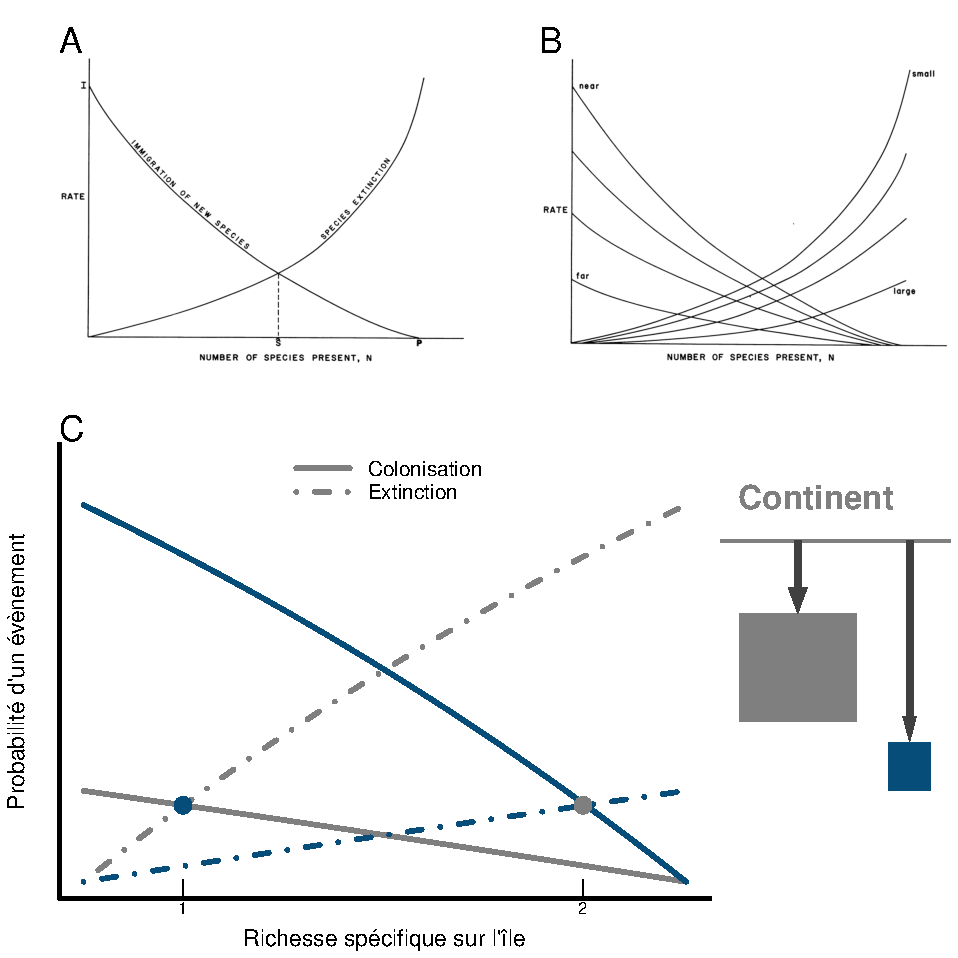
\includegraphics{fig/fig1.pdf}
\caption{\textbf{La Théorie de la biogéographie des Iles.} (A) illustre
l'évolution des taux de colonisation et d'extinction est présentée pour
deux îles aux caractéristiques différentes. Les tailles relatives des
îles et les distances qui les séparent du continent sont schématisées
sur la droite, les couleurs associent les îles à leurs courbes
respectives. Le réservoir d'espèce régional (\(P\)) est constitué de 100
espèces, les taux de colonisation et d'extinction sont exprimés en terme
de probabilité d'évènement (de colonisation ou d'extinction). Les points
marquent les intersections entre les courbes d'extinction et de
colonisation c'est-à-dire lorsque ces processus s'équilibrent.
L'abscisse de ces point indique les richesses spécifiques de l'île à
l'équilibre \(S_{eq}\). (B) et (C) sont respectivement les figures 4 et
5 extraites de l'article de 1963 de MacArthur et Wilson qui livre
essentiellement le même message que celui illustré en (A)
\citep{MacArthur1963}. La forme convexe des courbes de 1963 sont
justifiées par des facteurs biologiques qui ne sont pas intégrés dans
l'équation \label{eqMW} qui confère une forme concave aux courbes comme
vu en (A).\label{fig:figMW}}
\end{figure}
%
\subsection*{L'importance de la TIB dans des développements théoriques
plus
récents}\label{limportance-de-la-tib-dans-des-duxe9veloppements-thuxe9oriques-plus-ruxe9cents}
\addcontentsline{toc}{subsection}{L'importance de la TIB dans des
développements théoriques plus récents}

\subsubsection*{La théorie des
métapopulations}\label{la-thuxe9orie-des-muxe9tapopulations}
\addcontentsline{toc}{subsubsection}{La théorie des métapopulations}

Bien que ne représentant que cinq pour-cents des terres émergées, ce
sont bien les observations de la faune des îles qui ont mené à une
vision paradigmatique de la biogéographie. L'importance des îles
s'expliquent par leur relative abondance, leur disparité, leur
diversité, la relative simplicité des assemblages biologiques qu'on y
trouve et aussi, comme je l'ai évoqué précédemment, par la clarté des
flux de migrations \citep{Simberloff1974a}. Cette dernière propriété est
souvent absente pour des populations continentales\footnote{Les îles
  sont cependant souvent dans des archipels où la lecture de ces flux
  n'est pas si simple.}. La théorie des métapopulations s'intéresse
justement aux populations reliées entre elles par des flux de migrations
\citep{Hanski2010}. Le premier modèle de métapopulations a été proposé
par Levins\footnote{Richard Levins qui avec Heatwole est un des
  co-découvreurs des idées de la TIB.} lors d'une réflexion sur le
contrôle démographique des ravageurs dans les cultures
\citep{Levins1969}. Pour un ravageur donné, les îlots de culture sont
autant de patchs où une population peut se maintenir et disperser dans
les autres patchs alentour. Levins montre alors que les mesures de la
lutte biologique doivent être conduites à large échelle pour en
augmenter les probabilités de succès, c'est-à-dire d'extinction régional
du ravageur~\citep{Levins1969}. Le modèle est simple et très proche de
celui de la TIB : l'évolution de la proportion \(p\) est aussi gouvernée
par des évènements de colonisation \(c\) et d'extinction \(e\) :

\begin{eqnarray}
\label{eqMW}
\frac{dp}{dt} = cp(1-p)-ep
\end{eqnarray}

La différence fondamentale avec la TIB est que la migration dépend de la
proportion de patchs occupés : plus elle est importante plus la
migration est importante. Parmi les démonstrations il y a les travaux
menés notamment par Ikkha Hanski sur les population du Mélitée du
plantain (\emph{Melitaea cinxia}) au sud-ouest de la Finland
\citep{Hanski1998}. En plus de données un cadre de penser plus réaliste
en terme de configuration spatiale, les dynamiques populationnelles
associées sont bien comprises et mènent à des risques d'extinction mieux
évalués \citep{Hanski1998}. C'est aussi un cadre approprié pour insérer
l'étude des flux génétiques liés à l'arrangement spatial des
populations. Ainsi, toujours sur ces mêmes populations de papillon, Ilik
Saccheri et collègues montrent qu'en ajoutant le degrés d'hétérozygotie,
ils obtiennent des prédictions précises quant l'extinction locale des
populations \citep{Saccheri1998}. Les travaux théoriques autour du
concept de metapopulations proposent un certain nombre de paradigmes qui
permettent d'évaluer le rôle que je joue les processus de colonisation
et d'extinction dans les variations spatio-temporelles de la démographie
d'une espèce \citep{Leibold2004}. La prépondérance de ces mécanismes qui
font la force de la TIB et de la théorie des métapopulations a été
poussée à son paroxysme dans la théorie neutre de la biogéographie.

\subsubsection*{La théorie neutre de la biogéographie et le débat
qu'elle
soulève}\label{la-thuxe9orie-neutre-de-la-bioguxe9ographie-et-le-duxe9bat-quelle-souluxe8ve}
\addcontentsline{toc}{subsubsection}{La théorie neutre de la
biogéographie et le débat qu'elle soulève}

La théorie neutre postule l'équivalence écologique entre les différents
individus d'espèces éventuellement différentes et décrit les dynamiques
populationnelles reposant sur les différences d'abondance relative à
l'échelle régionale et locale. Ainsi, en 1997, dans l'article fondateur
de la théorie neutre, Stephen Hubbell décrit un modèle dans lequel le
replacement d'un individu mort dans une communauté locale est le
résultat d'un tirage aléatoire : le nouvel individu peut soit être
recruté localement et la probabilité que l'individu soit d'une espèce
donnée dépend de l'abondance relative de cette dernière dans la
communauté locale soit le nouvel individu peut-être un immigrant dont
l'identité de l'espèce à laquelle il appartient est liée à l'abondance à
l'échelle régionale de celle-ci \citep{Hubbell1997}. En plus des
exemples donnés dans l'article de 1997, Hubbell montre de manière
convaincante que dans la forêt tropical du Panama, à la suite d'un
chablis, le recrutement de l'arbre n'est pas prévisible par ces
caractéristiques et que le recrutement est similaire à la composition
alentour \citep{Hubbell1999}. La dynamique engendrée est appelée la
dérive écologique, elle dominée par la stochasticité qui conduit presque
certainement à l'extinction de toutes les espèces sauf une, ce qui est
contrebalancée par l'apparition d'espèces nouvelles
\citep{Hubbell2010, Ricklefs2003}.

La théorie neutre partage beaucoup de caractéristiques avec la TIB : les
mécanismes fondamentaux sont l'extinction et la colonisation,
l'hypothèse d'équivalence écologique et l'imbrication des échelles
régionales et locales. Comme le fait remarquer Hubbell en 2010 dans le
chapitre qu'il écrit dans \emph{The Theory of Island Biogeography
Revisited}, la théorie neutre place l'équivalence écologique au niveau
des individus et non plus au niveau des espèces \citep{Hubbell2010}. Une
conséquence directe revendiquée par Hubbell est que cette hypothèse
explique la forme convexe des courbes de colonisation et d'extinction
décrites par MacArthur et Wislon mais que n'explique pas leur modèle
(voir \ref{fig:figMW} et \citet{Hubbell2010}). Le principe d'équivalence
et la place importante que prend le hasard dans cette théorie a soulevé
de très vif débats et des démonstrations à charge contre la véracité de
la théorie (voir par exemple \citet{McGill2003} et
\citet{Ricklefs2003}). L'équivalence écologique doit, à mon sens, être
comprise comme une abstraction de la singularité des espèces, une
simplification de la diversité des systèmes biologiques, nécessaire à
l'isolation d'une portion restreinte des phénomènes en cause dans la
répartition géographique des espèces pour en évaluer le pouvoir
explicatif. Bien qu'un certain nombre de cas d'études permettent de
rejeter cette théorie \citep{McGill2003, John2007}, les défenseurs de la
théorie neutre affirment qu'elle est tout aussi utile quand une étude en
démontre la fausseté \citep{Rosindell2012}. La théorie neutre peut en
effet être présentée comme une jauge qui mesure sur l'importance des
processus de différentiation de niches \citep{Wennekes2012}. Ainsi, pour
certaines communauté la dérive écologique est plus importante que dans
d'autre et du point du vue de formalisme des solutions ont déjà été
proposée pour dresser un continuum de la théorie neutre vers la théorie
de la niche écologique \citep{Gravel2006a}. Malgré les possibilités
offertes par ces deux théories, elles occultent largement les
interactions écologiques qui sont factuelles; si les observations
donnent crédit à ces théories, une théorie intégrative de la
biogéographie doit expliquer pourquoi.
%
\section*{Le rôle des interactions dans la distribution des
espèces}\label{le-ruxf4le-des-interactions-dans-la-distribution-des-espuxe8ces}
\addcontentsline{toc}{section}{Le rôle des interactions dans la
distribution des espèces}

Ma thèse a pour objectif de trouver des leviers pour intégrer les
interactions écologiques dans la TIB et comprendre comment elles
affectent la répartition géographique des espèces et de comprendre où
chercher les traces qu'elles pourraient éventuellement laisser dans les
données d'occurrence des espèces. Comme je l'ai mentionné plus haut
cette idée est très ancienne, Wallace le remarque dans son livre publié
en 1881:

\begin{quote}
« Both compétition and predation appear now to be much more important in
biogeography than people had formely guesses »
\end{quote}

Le problème de ces relations écologiques est leur spécificité, l'unicité
de chacune d'entre elles, dont découle nos difficultés pour les prévoir
bien que des travaux récents explorent des pistes prometteuse pour les
prédire notamment sur la base de relations allométriques entre proie et
prédateur \citep{Gravel2013}. Au point de vue théorique et à l'examen
des chapitres du dernier livre de MacArthur
\citep{macarthur1972geographical}, il apparait que l'intégration des
interactions est une étape clef pour aller vers une biogéographie
intégrative et c'est dans cette direction que j'ai mené ma thèse, en
essayant d'apporter des pistes pour arriver à une telle intégration.

\subsection*{Importance des interactions dans la
distribution}\label{importance-des-interactions-dans-la-distribution}
\addcontentsline{toc}{subsection}{Importance des interactions dans la
distribution}

Dans la théorie de la biogéographie des îles, les interactions sont en
fait omniprésentes car elles sont une des composantes principales du
processus d'extinction. Cependant, dans la formulation du modèle, elles
ne sont jamais mentionnées explicitement, cachés dans le taux
d'extinction \(e\). Comme je le montre à la figure \ref{fig:figMW}, la
différence dans l'allure des courbes dessinées par MacArthur et Wilson
et celles obtenues en supposant un taux d'immigration et de colonisation
sont différentes. D'après les auteurs, l'immigration devient plus
difficile lorsque les espèces s'accumulent sur l'île et les extinctions
sont de plus en plus fréquentes dues à l'intensification des
interactions. Pour parler en terme de réseau d'interaction,
l'accumulation d'espèces sur l'île sature le réseau local et rend
difficile l'intégration d'une nouvelle espèce qui le rend par ailleurs
de plus en plus instable. Une interprétation en terme de communauté de
la TIB est tout à fait possible mais les liens entre les espèces ne sont
pas formulés mathématiquement en 1967.

Depuis les années 60, la littérature théorique n'a cessé de discuter le
rôle joué par les interactions intra- et inter-spécifiques dans la
distribution spatiale des espèces. Il est reconnu que l'interdépendance
des espèces détermine le caractére favorable de l'environnement au sens
large (biotique et abiotique). En 2009, Robert Holt et Michael Barfield
discutent de l'impact de la prédation sur la répartition d'espèces en
compétition insistant alors sur le rôle majeur des interactions dans le
dessin des aires de répartition \citep{Holt2009}. En 2012, William
Godsoe et Luke Harmon Godsoe introduisent les interactions dans un
modèle simple de distribution d'espèce et montre comment la probabilité
de présence d'une espèce peut être affectée par la distribution d'une
seconde et concluent alors que cela doit affecter vraisemblablement la
qualité de prédictions des SDMs \citep{Godsoe2012}. La remise en cause
actuelle de ces modèles est une étape fondamentale car leur succès
depuis la fin du siècle dernier a relégué les interactions écologiques
au second plan en démontrant que la corrélation avec les variables
climatiques étaient peut-être suffisante, au moins en première
approximation pour expliquer les aires de répartitions
\citep{Pearson2003}. Pourtant, dès 1998, le travail précurseur d'Andrew
Davis et collègues \citep{Davis1998} avait fortement remis en question
l'hypothèse d'indépendance des espèces \citep{Jeschke2008}. L'expérience
dont les résultats sont publiés en 1998 est une analyse d'abondance de
trois espèces de drosophile le long d'un gradient de température. Les
comparaisons d'abondance sont menées pour toutes les combinaisons
possibles de ces trois mouches (assemblages à 1, 2 ou 3 espèces) mais
aussi en présence ou en absence d'un parasitoïdes. La démonstration est
sans appel, la compétition et parasitisme affectent drastiquement la
survie le long du gradient de température, les interactions affectent
donc très probablement les réponses au changement climatique.

Plus récemment, on constate une grande motivation pour intégrer les
relations écologiques dans les modèles de distribution d'espèces
\citep{Kissling2012, Guisan2011}. Une méthodologie récente appelée JSDM
intègre les corrélations dans la présence des espèces pour améliorer les
prédictions \citep{Pollock2014}. Néanmoins, ces efforts se heurtent à un
manque de maturité des modèles et théories qui cherchent à rassembler
distribution et interactions. Parmi les travaux récents, Franck Jabot et
Jordi Bascompte ont rassemblé metacommunauté et écologie des réseaux
souligner importance des relations écologiques dans la répartition
géographique des espèces \citep{Jabot2012}. De même, Dominique Gravel et
collègues introduisent en 2011 l'interdépendance proie-prédateur dans le
modèle de la TIB menant aux prémices d'une théorie trophique de la
biogéographie des îles \citep{Gravel2011} préfigurée par Holt
\citep{Holt2009a}. Ces travaux essayent de dépassés l'hypothèse
d'équivalence écologique en vue de faire des prédictions plus précise
sur les compositions spécifique attendues localement.

C'est dans la lignée de ces développements théoriques récents que
s'inscrit mon premier chapitre de thèse. J'y ai montré comment
l'intégration du concept de réseau écologique dans la TIB était possible
tout en ajoutant la reconnaissance de performances plus ou moins
importantes des espèces dans un contexte abiotique donné (niche
écologique). Pour y arriver, j'ai montré l'interêt de considérer les
espèces sous la forme d'assemblage plutôt que une à une. Du point de vie
technique, mon travail montre aussi qu'un retour aux processus
stochastiques tels que ceux présentés en 1967 est une démarche puissante
pour ajouter de nouveaux mécanismes dans la TIB.

\begin{figure}[htbp]
\centering
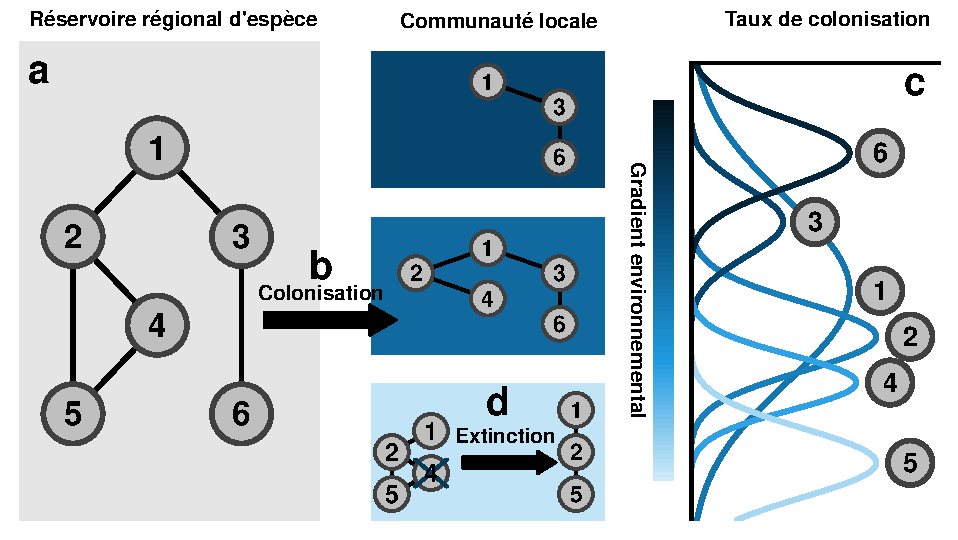
\includegraphics{fig/fig2.pdf}
\caption{\textbf{Intégration des interactions et des contraintes
abiotiques dans la TIB.} Pour intégrer les interactions j'ai considéré
non pas un ensemble d'espèces indépendant mais des espèces au sein d'un
réseau décrit à l'échelle régional (a). Comme dans la TIB ces espèces
peuvent être colonisée l'île (b), mais dans le modèle que j'ai
développé, les taux de colonisation varient avec le long d'un gradient
environnemental (c). Enfin, les interactions influencent les taux
d'extinction locaux (d).\label{fig:figGTIB}}
\end{figure}

\subsection*{Un problème d'échelle?}\label{un-probluxe8me-duxe9chelle}
\addcontentsline{toc}{subsection}{Un problème d'échelle?}

En repartant de l'exemple classique de la ségrégation spatiale des
tamias \emph{Eutamias dorsalis} et \emph{E. umbrinus} \citep{Brown1971},
j'ai précédemment mis en évidence qu'une information sur les
interactions est contenue dans les aires de répartitions de ces espèces.
Il y a cependant deux caractéristiques qui peuvent conduire à la rareté
de ce type de lecture : la singularité de l'interaction et son caractère
locale. Je reviens un peu plus bas sur la première propriété et m'arrête
ici sur la seconde. Une idée dominante en biogéographie est que les
interactions ont des rôles majeurs à l'échelle locale mais que leurs
conséquences sont de moins en moins perceptible à mesure que l'on
considère des échelles spatiales de plus en plus grandes (voir l'unique
figure de \citet{McGill2010}). Du point de vue théorique, c'est tout à
fait ce qui est décrit dans la TIB car c'est à l'échelle locale que les
interactions influencent l'extinction. Néanmoins, ces conséquences
locales sont présentent sur l'ensemble de la distribution de l'espèce,
il est alors pertinent de se demander pourquoi nous ne sommes pas
capables de détecter les interactions en examinant les distributions
d'espèces. En réalité, bien que cela soit rare, nous avons des preuves
que cela est possible dans certains cas. En 2010, Nicholas Gotelli et
collègues divisent l'avifaune danoise en différentes catégories fondées
sur la similarité écologique et démontrent que les espèces d'une même
catégorie sont très souvent significativement spatialement ségréguées
\citep{Gotelli2010}. De même, en 2007, Risto Heikkinen et collègues
avaient obtenu des performances accrues de leurs modèles statistiques
par l'utilisation de la répartition de six espèces de pics pour
expliquer la présence de quatre espèces de hiboux \citep{Heikkinen2007}.
Dans cette même étude, le signal est plus fort quand les données sont
sur de 10x10km que 40x40km en faveur d'une dépendance à l'échelle,
récemment supportée par d'autres travaux \citep{Belmaker2015}. Ce qui
est remarquable dans les travaux de Gotelli et de Heikkinen est que
l'utilisation d'une connaissance biologique et écologique a permis de
révéler une trace des interactions dans la distribution d'espèces.

La dépendance spatiale de la détection des interactions est facile à
comprendre : en examinant des données de présence à des échelles
spatiales de plus en plus larges, le nombre d'espèces s'accumule (c'est
le principe de la relation aire-espèce) menant à la dégradation de
l'information potentielle. Cela signifie que l'information nécessaire
pour déceler des empreintes laissées par les interactions sera fournit
par des données à l'échelles relativement fine. Cependant, cela ne
permet pas de conclure sur le rayon d'action de ces interactions. Pour
dépasser la question spatiale, il fait aussi envisager l'impact de la
nature des interactions sur la répartition géographique. Ainsi, en 2014,
Miguel Araújo et Alejandro Rozenfeld ont prouvé théoriquement que les
interactions positives (mutualisme) se propageaient davantage que les
interactions négatives \citep{Araujo2014}. Par conséquent, la nature de
la relation qui unit des espèces peut influencer la perte d'information
contenue dans les aire de répartition. Suite à mes travaux sur
l'intégrations des interactions, je me suis penché sur un autre aspect
qui peut influencer la perte d'information dans les données de présence
: l'abondance des interactions. Au chapitre 2, je montre que les
interactions directes et indirectes affectent les données de
distributions mais aussi que l'abondance des interactions rend difficile
de distinguer la co-occurrence d'espèces en interactions d'une
co-occurrence aléatoire. Ce qui est encore plus intéressant, c'est que
j'ai accumulé un certain nombre d'indices dans des données de présence
et d'absence réelle qui semblent confirmer nos prédictions. Je discute
de ces résultats dans le troisième chapitre de ma thèse.

En constatant que l'abondance des interactions peut justifier
l'hypothèse d'indépendance des espèces, je soulève le même paradoxe que
celui relevé par MacArthur dans son oeuvre de 1972
\citep{macarthur1972geographical} :

\begin{quote}
« A few decades ago it as fashionable for ecologist to study communities
in the arctic on the grounds that these would be very simple communities
and hence easy to understand. Many excellent ecologists still follow
this belied, but there are others who feel that it may be easier to
understand the extremely complex communities. This sounds paradoxical:
How can a more complex communities by easier to understand? A possible
answer might be that complex community has has strong interactions among
species so that the lives of the separate species are less independent
than in a simple community. Where there is greater interdependence,
patterns may be more conspicuous. »
\end{quote}

Encore une fois, je déplace le problème car si l'interdépendance est
importante pour des système simple, le problème est de prédire quand ces
systèmes le sont. Autrement dit, il serait peut-être pertinent de situer
les prédictions en biogéographie au niveau du réseau écologique. Le
problème d'échelle n'est plus seulemnt spatial et temporel il est aussi
un problème d'échelle biologique : individus, population, communauté ou
réseaux?

\subsection*{Vers une biogéographie
énergétique}\label{vers-une-bioguxe9ographie-uxe9nerguxe9tique}
\addcontentsline{toc}{subsection}{Vers une biogéographie énergétique}

Le problème d'échelle biologique est aussi un problème de catégorisation
des espèces. J'ai suggéré que les prédictions étaient plus faciles pour
des espèces généralistes que pour des espèces spécialistes.
Malheureusement, le spectre est très large et plutôt balancé avec un
continuum entre des espèces hyperspécialistes de d'autres très
généralistes \citep{Poisot2015c}. On peut néamoins espérer que la
réduction des espèces à un certains nombres de traits
\citep{McGill2006, Poisot2015} doublée d'une réduction des des réseaux à
un certains nombre de propriétés puissent permetre des généralisations
utiles dans notre compréhension de la distribution des communautés. Il
m'apparaît aujourd'hui urgent que le niveau bon niveau de détail dans
nos descriptions des systèmes écologiques soit trouvé afin de renforcer
les fondements théoriques de la dynamique des aires de répartitions.

Une piste prometteuse pour prolonger la recherche des propriétés est me
semble-t-il de s'appuyer sur la nature profonde des espèces : des
systèmes énergétiques qui se perpétuent. La lecture de la théorie de la
dynamique du budget énergétique de Sebastian Kooijman
\citep{Kooijman2000a} m'a été très profitable pour cerner les
possibilités offertes par une telle approche. S'il est possible, comme
le suggèrent les travaux de Kooijman, de dériver de manière précise un
grande nombre de propriétés énergétiques des espèces sur leur masse et
leur forme, alors les espoirs sont grands de pouvoir trouver des règles
d'assemblages fiables des communautés et donc de comprendre d'un point
de vue mécaniste les extinctions locales. Ce sont les mêmes espoirs que
ceux nourrit par la théorie métabolique de l'écologie qui rassemble des
relations entre la taille des espèces et différentes de leurs propriétés
\citep{Brown2004} qui montrent en somme qu'il est possible d'aller
au-delà de l'espèce \citep{Poisot2015}. Mes réflexions sur
l'intersection entre la TIB et une vision énergétique de l'écologie sont
présentées au chapitre 4 de ma thèse, dans un chapitre qui se veut aussi
comme une ouverture vers les projets de recherche que j'aimerais mener
dans un futur proche.
